\section{Le stage dans ses grandes lignes}
\begin{frame}
	\tableofcontents[currentsection]
\end{frame}

	\subsection{Bruteforce}
	\begin{frame}{Fonctionnement}{\textbf{Exemple :} Polybridge}
		\begin{figure}
			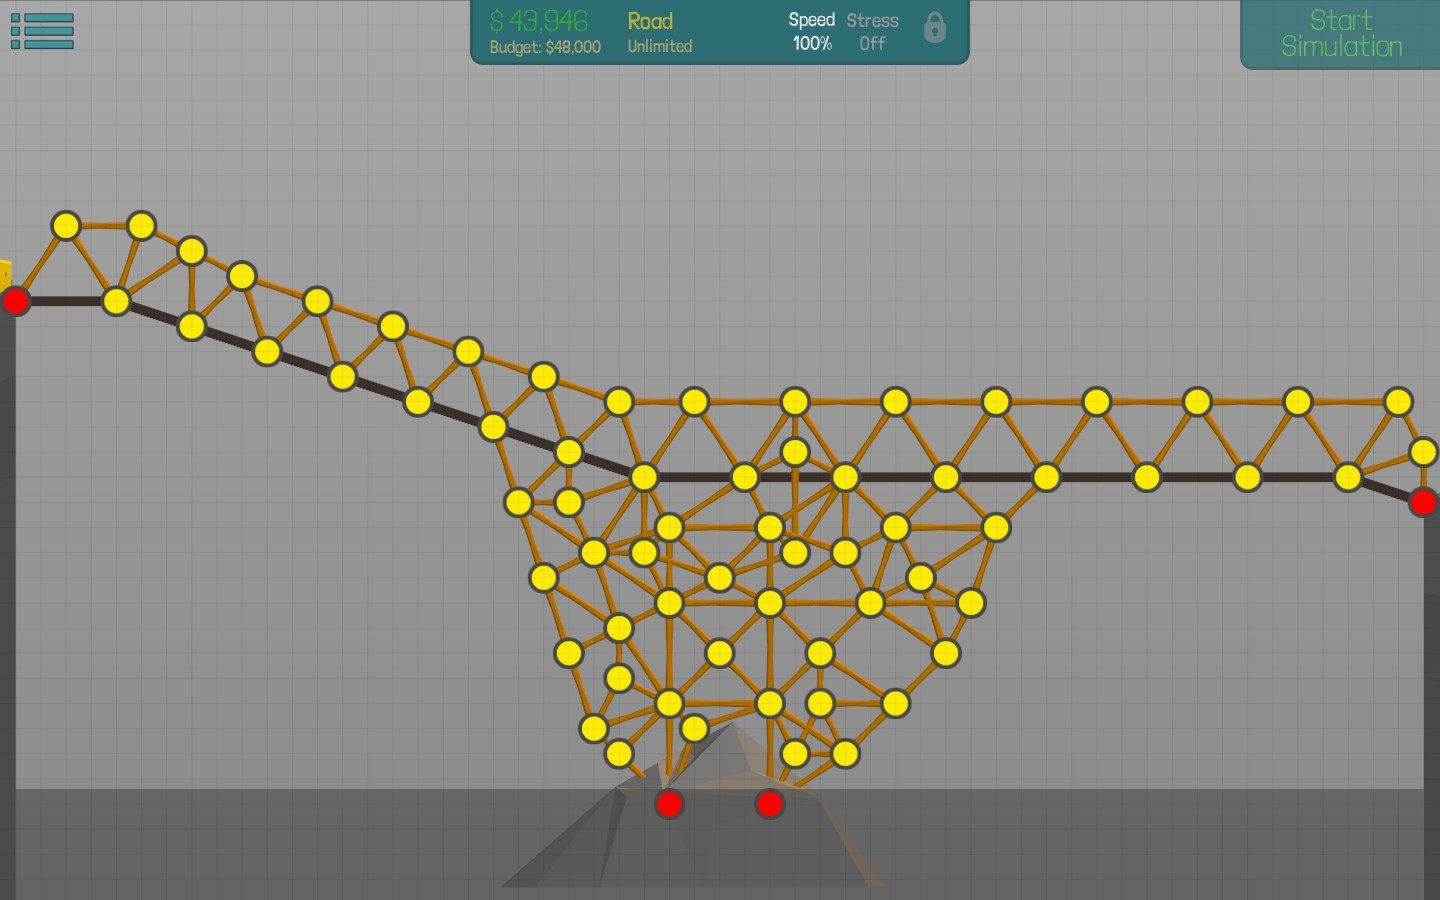
\includegraphics[width=0.9\textwidth]{images/polybridge_bruteforce}
		\end{figure}
	\end{frame}
	\begin{frame}[plain]{Différents parcours}
			\begin{figure}[H]
				\minipage{0.32\textwidth}
				\textbf{rowscan}
				
				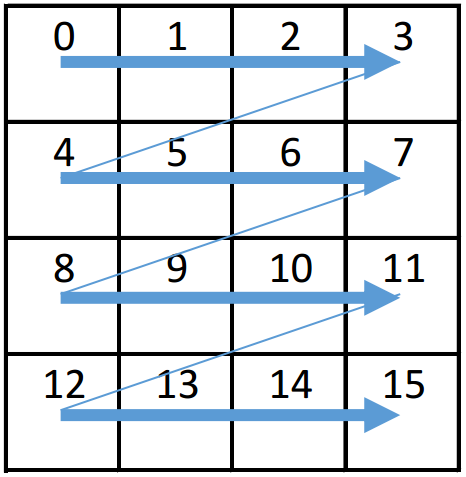
\includegraphics[width=\linewidth]{images/parcours_rowscan.png}
				\endminipage\hfill
				\minipage{0.32\textwidth}
				\textbf{diagonal}
								
				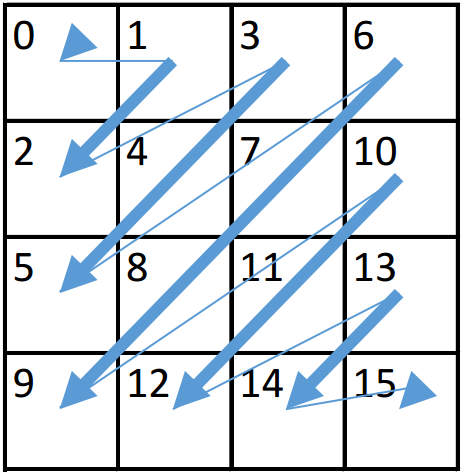
\includegraphics[width=\linewidth]{images/parcours_diagonal.png}
				\endminipage\hfill
				\minipage{0.32\textwidth}
				\textbf{spiral--in}
				
				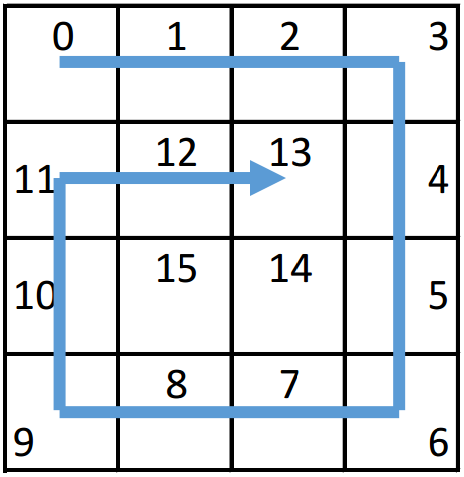
\includegraphics[width=\linewidth]{images/parcours_spiral-in.png}
				\endminipage\hfill
				\minipage{0.32\textwidth}
				\textbf{spiral--out}
				
				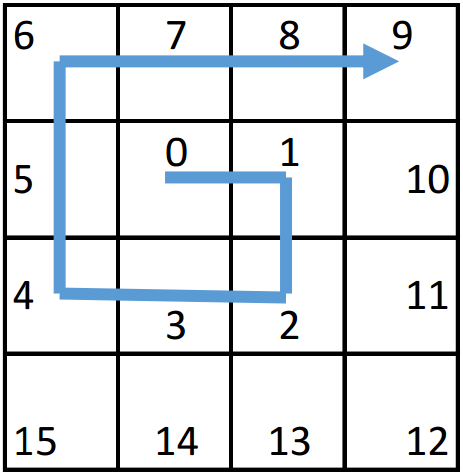
\includegraphics[width=\linewidth]{images/parcours_spiral-out.png}
				\endminipage\hfill
				\minipage{0.32\textwidth}
				\textbf{quad--spiral--in}
				
				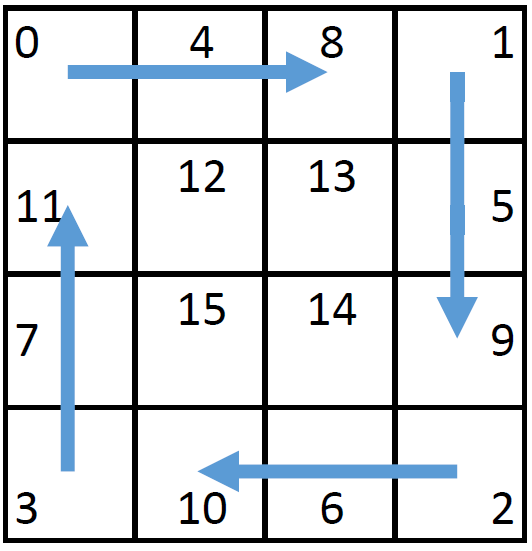
\includegraphics[width=\linewidth]{images/parcours_quad-spiral-in.png}
				\endminipage\hfill
				\minipage{0.32\textwidth}
				\ %don't touch this !
				\endminipage\hfill
			\end{figure}
	\end{frame}
	\begin{frame}{Résultats}
		\begin{figure}
			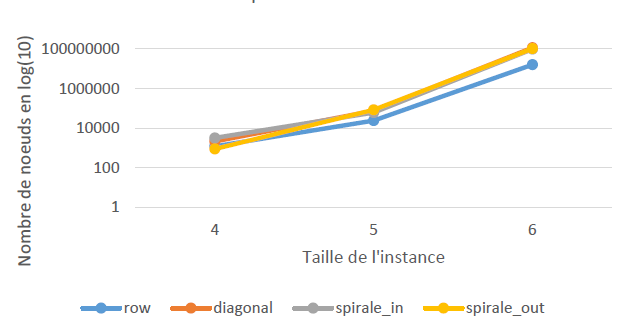
\includegraphics[width=\textwidth]{images/resultat_bruteforce_graphique_all}
		\end{figure}
	\end{frame}
	\subsection{Smartforce}
	\begin{frame}{Structurer les différentes visions du jeu}
		\begin{itemize}[<+->]
			\item Cases/Pièces (CaPi) vision par défaut.
			\only<1>{
\includegraphics{images/matching_pieces}}
			\item Bordures/Couleurs (BoCo).
			
			\only<2>{\includestandalone[mode=image,width=0.5\textwidth]{graphics/boco}}
			\item Bordures/Couleurs Diagonale (BoCoDiag)
			\only<3>{
				\begin{minipage}{0.46\textwidth}
					\includestandalone[mode=image,width=\textwidth]{graphics/bocodiag}
				\end{minipage}\hfill
				\begin{minipage}{0.46\textwidth}
					\includestandalone[mode=image,width=\textwidth]{graphics/bocodiag_abstract_1}
				\end{minipage}\hfill
				}
		\end{itemize}
	\end{frame}
	
	\subsection{Conclusion}
	
	\begin{frame}{En quelques chiffres}
		%TODO
	\end{frame}
	
	\begin{frame}
		\begin{figure}
			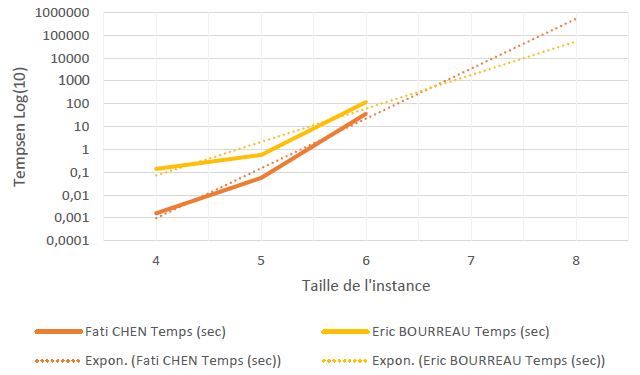
\includegraphics[width=\textwidth]{images/resultat_bruteforce_rowscan}
		\end{figure}
	\end{frame}